\documentclass[border=4pt]{standalone}
\usepackage{amsmath,amssymb,tikz}
\usetikzlibrary{arrows.meta}
\definecolor{figB}{RGB}{31,90,166}\definecolor{figR}{RGB}{176,48,48}
\begin{document}
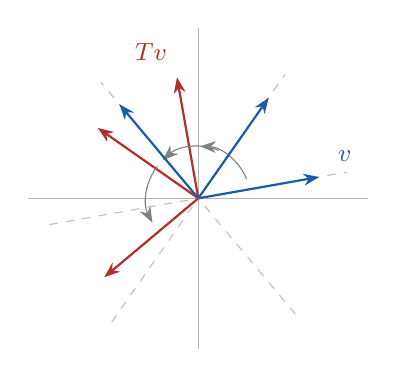
\begin{tikzpicture}[scale=1.2,>={Stealth[length=2mm]}]
\draw[gray!60] (-1.8,0)--(1.8,0); \draw[gray!60] (0,-1.6)--(0,1.8);
\foreach \a in {10,55,130} {
  \draw[dashed,gray!50] ({-1.6*cos(\a)},{-1.6*sin(\a)})--({1.6*cos(\a)},{1.6*sin(\a)});
  \draw[->,thick,figB] (0,0)--({1.3*cos(\a)},{1.3*sin(\a)});
  \draw[->,thick,figR] (0,0)--({1.3*cos(\a+90)},{1.3*sin(\a+90)});
  \draw[->,gray,thin] ({0.55*cos(\a+12)},{0.55*sin(\a+12)}) arc ({\a+12}:{\a+78}:0.55);
}
\node[figB,font=\small] at (1.55,0.45) {$v$};
\node[figR,font=\small] at (-0.5,1.55) {$Tv$};
\end{tikzpicture}
\end{document}
